\begin{tikzpicture}[
    cell/.style={draw, minimum width=1.5cm, minimum height=0.8cm, font=\small},
    feat_label/.style={font=\tiny, gray, align=center}
]
\node[cell, fill=irSparse!20] (c1) {$x_1$};
\node[cell, fill=irSparse!20, right=0cm of c1] (c2) {$x_2$};
\node[cell, fill=irSparse!20, right=0cm of c2] (c3) {$x_3$};
\node[cell, fill=irSparse!20, right=0cm of c3] (c4) {$\dots$};
\node[cell, fill=irSparse!20, right=0cm of c4] (c5) {$x_n$};

\node[below=0.1cm of c1, feat_label] {BM25\\Score};
\node[below=0.1cm of c2, feat_label] {PageRank};
\node[below=0.1cm of c3, feat_label] {Click\\Count};
\node[below=0.1cm of c5, feat_label] {Freshness};

\node[left=0.5cm of c1, font=\normalsize] {$\Phi(q, d) = $};
\draw[decorate, decoration={brace, amplitude=10pt, mirror}, thick] ($(c1.south west)+(0,-0.6)$) -- ($(c5.south east)+(0,-0.6)$) node[midway, below=12pt] {$\mathbf{x}_{q,d} \in \mathbb{R}^{1000+}$};
\end{tikzpicture}

\vspace{1em}
\vspace{1em}
{\centering
\begin{tikzpicture}
    \IRBox{goal}{(0,0)}{The LTR Goal}{Learn $f(\mathbf{x}) \to \text{score}$ for optimal ranking}{hybrid}
\end{tikzpicture}
\par}
